\section{Databases}
Some databases has been used in order to learn, compare results and carry out the project. All the databases are formed by three subsets whose samples are not repeated among subsets: train, validation and test.

\begin{itemize}
\item The training subset is used to train the network during epochs. To know how the training behavior, a cost is calculated.
\item The validation subset is used to check the behavior of the network while is training, also, the validation subset is usually used to calculate the hyper-parameters of the network, although the hyper-parameters are not calculated until is pointed. The validation error is calculated for each training epoch. The metric use to the validation is $error(\%) = cost*100$.
\item  The test subset, that is used just at the end of the training. The best model is chosen with regard to the best validation error. Different metrics are going to be used for after testing the network (error rate(\%), TP, FP ...).
\end{itemize}

\subsection{MNIST digit database}\label{subsec:MNIST}
MNIST digit database is a image database of human written digits. This database is commonly used to learn machine learning techniques. Because of that, this database has been used, in this thesis, for learning Theano and convolutional neural networks. In addition, this database has been used in a implemented convolutional neural network (LeNet).\\
\begin{figure}[htb]
\centering
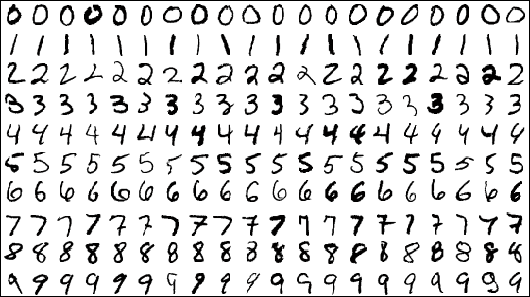
\includegraphics[width=0.6\textwidth]{images_databases/mnistExamples.png}
\caption{MNIST digit images database. Image obtained from \cite{MNISTimage}} \label{fig:MNIST_digits}
\end{figure}
Some examples of the digit image MNIST database could be seen in \ref{fig:MNIST_digits}, image obtained from \cite{MNISTimage} and the characteristics of this database are the following ones:

\begin{itemize}
 \item There are 70.000 number of unique samples.
 \item Altough original size of the database is 32x32 pixels, the samples of this downloaded database are 28x28 pixels in gray scale, that is 784 features per image.
 \item 10 classes could be differentiated, one per digit.
\item The samples are directly separated into train, test and validate subset.
\end{itemize}

\subsection{Labeled faces in the wild}
\textit{The Labeled Faces in the Wild} (LFW) is face database of well-known people that are collected from the net. The database can be found in its official web page \url{http://vis-www.cs.umass.edu/lfw/} \cite{LFWTech}.\\

The characteristics of this database are the following ones:
\begin{itemize}
 \item There are 13233 unique samples.
 \item The size of each image is 250x250 pixels. The number of features per image is 187500.
 \item There are images from 5748 different people, so there are 5748 different classes (if is used as one class per people).
\item The number of images per person is not the same for each one. There are 1680 people with two or more images.
\item The images are in RGB space.
\item The faces are centred in the image.\\
\end{itemize}
\begin{figure}[htb]
\centering
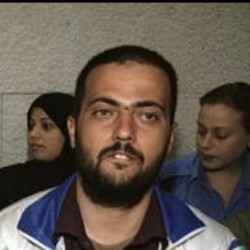
\includegraphics[width=0.2\textwidth]{images_databases/LFW/1.jpg}
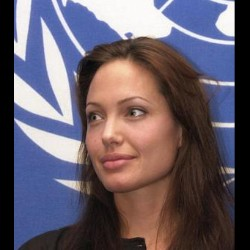
\includegraphics[width=0.2\textwidth]{images_databases/LFW/2.jpg}
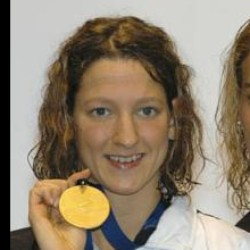
\includegraphics[width=0.2\textwidth]{images_databases/LFW/3.jpg}
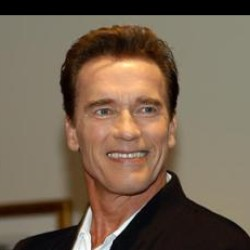
\includegraphics[width=0.2\textwidth]{images_databases/LFW/4.jpg}
\caption{Samples of LFW database} \label{fig:LFW1}
\end{figure}

Four examples of the images of this database could be seen in figure \ref{fig:LFW1} in which faces of well-known people are visualized.\\


This database has been used to learn; to learn how to read a database, how to feed the network with those images. It has been used assigning each class to a different people.\\

\subsection{FRAV dataset}
FRAV database is an anti-spoofing face database built in the FRAV research group of tu URJC University and which is part of the Automated Border Control Gates for Europe project \cite{ABC4EU}.\\

One exaple of RGB images of FRAV database are shown in figure \ref{fig:RGB-frav1} and another example could be seen in \ref{fig:RGB-frav2}. In both images, the four attacks described previously and the real user could be visualized. \\

\begin{figure}[htb]
\centering
\subfigure[printed image attack]{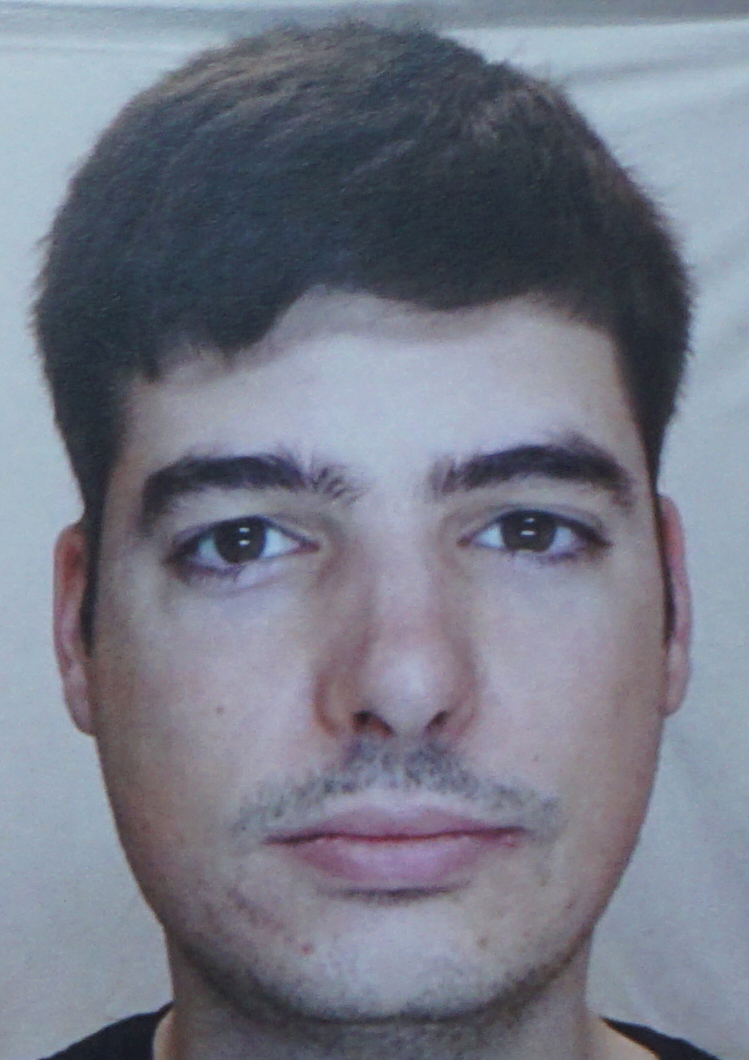
\includegraphics[width=0.18\textwidth]{images_databases/fravrgb/at1-0.JPG} \label{frav_im1-1} }
\subfigure[mask attack]{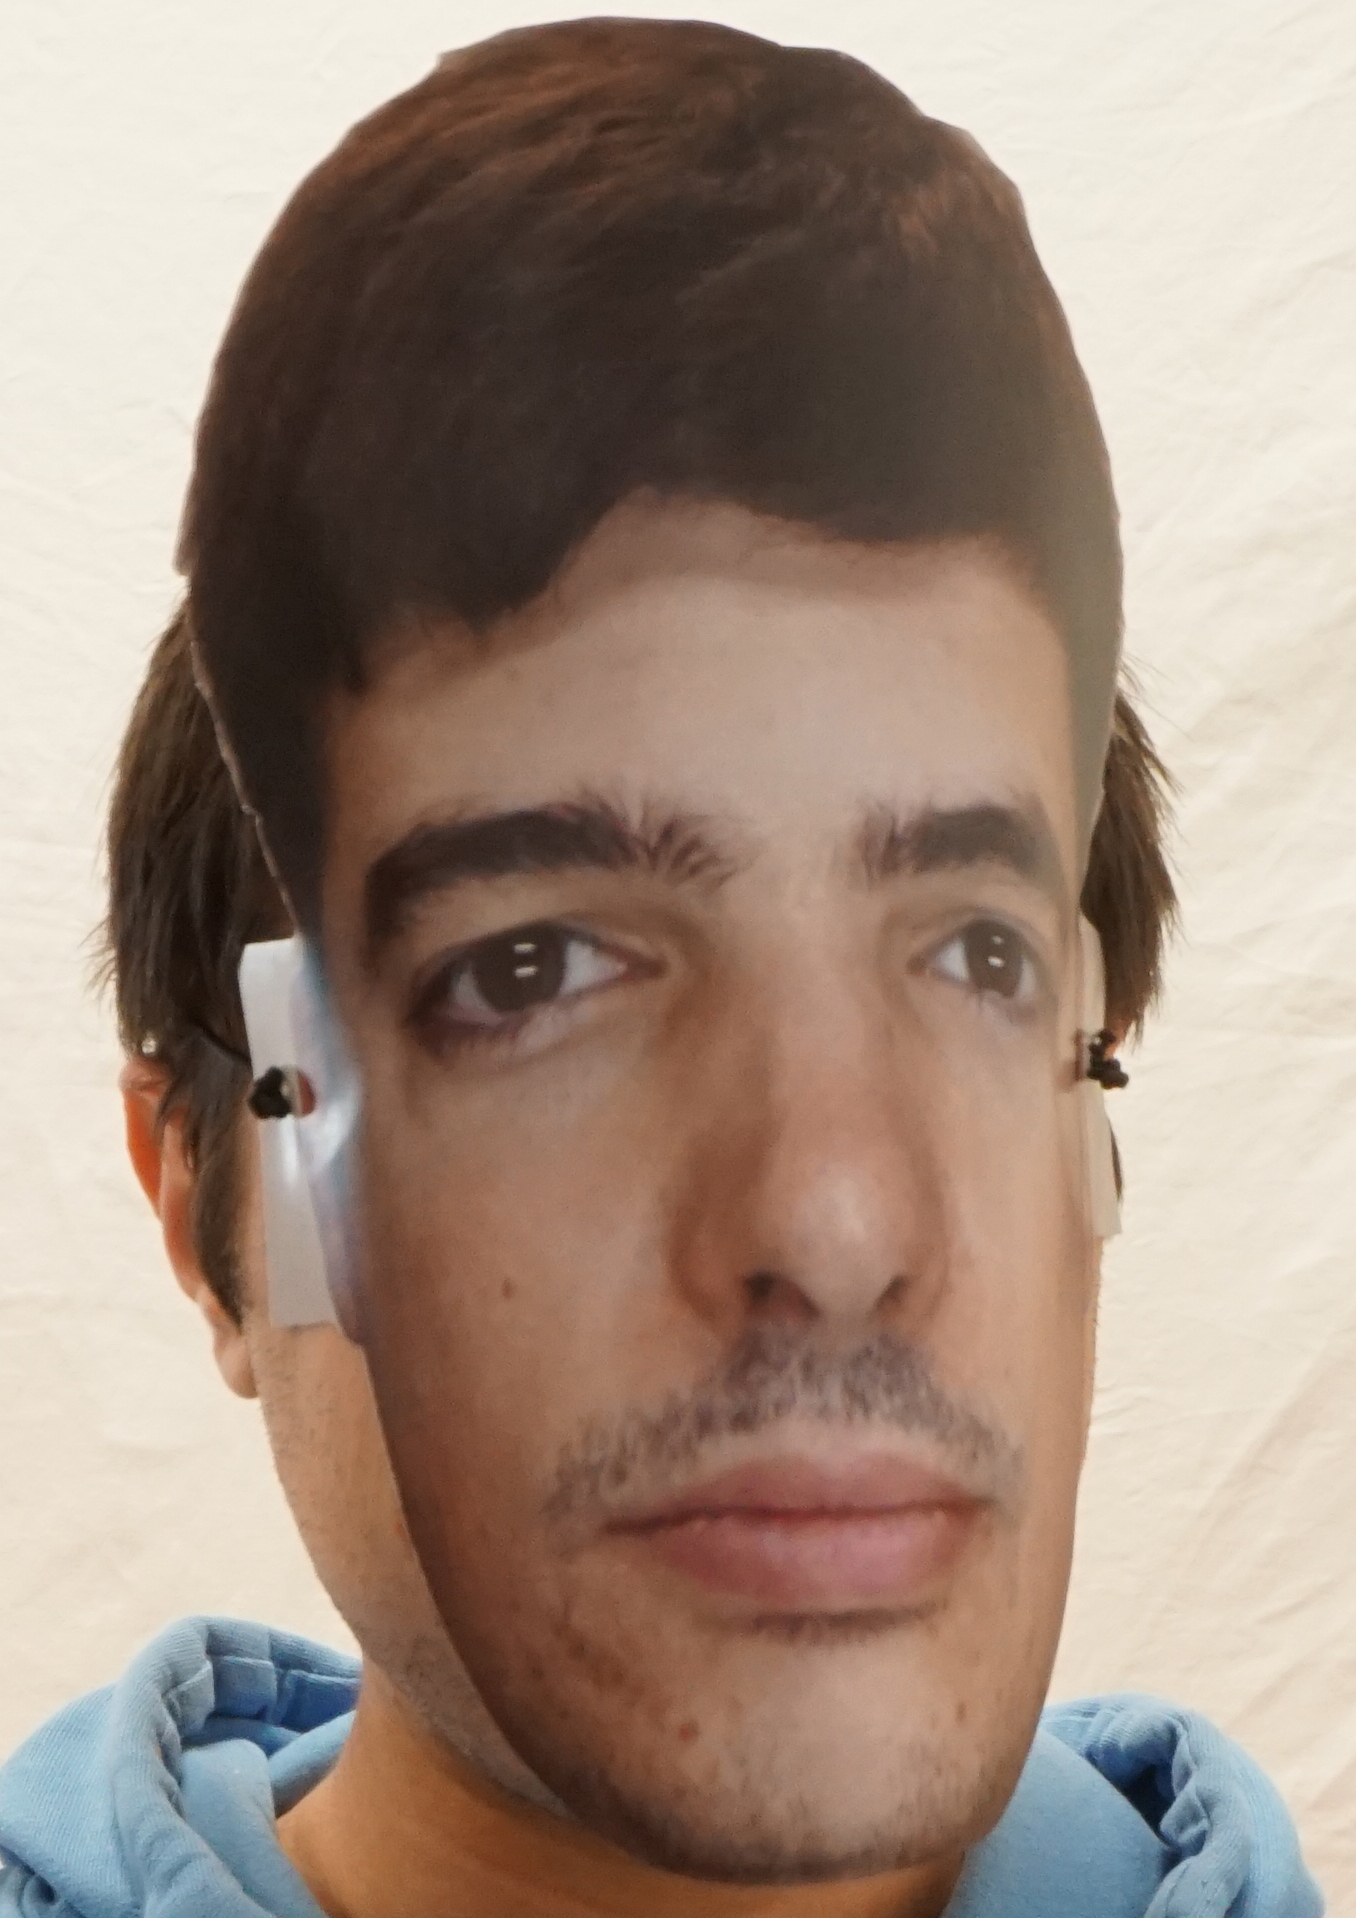
\includegraphics[width=0.18\textwidth]{images_databases/fravrgb/at2-0.JPG} \label{frav_im1-2}}
\subfigure[eye mask attack]{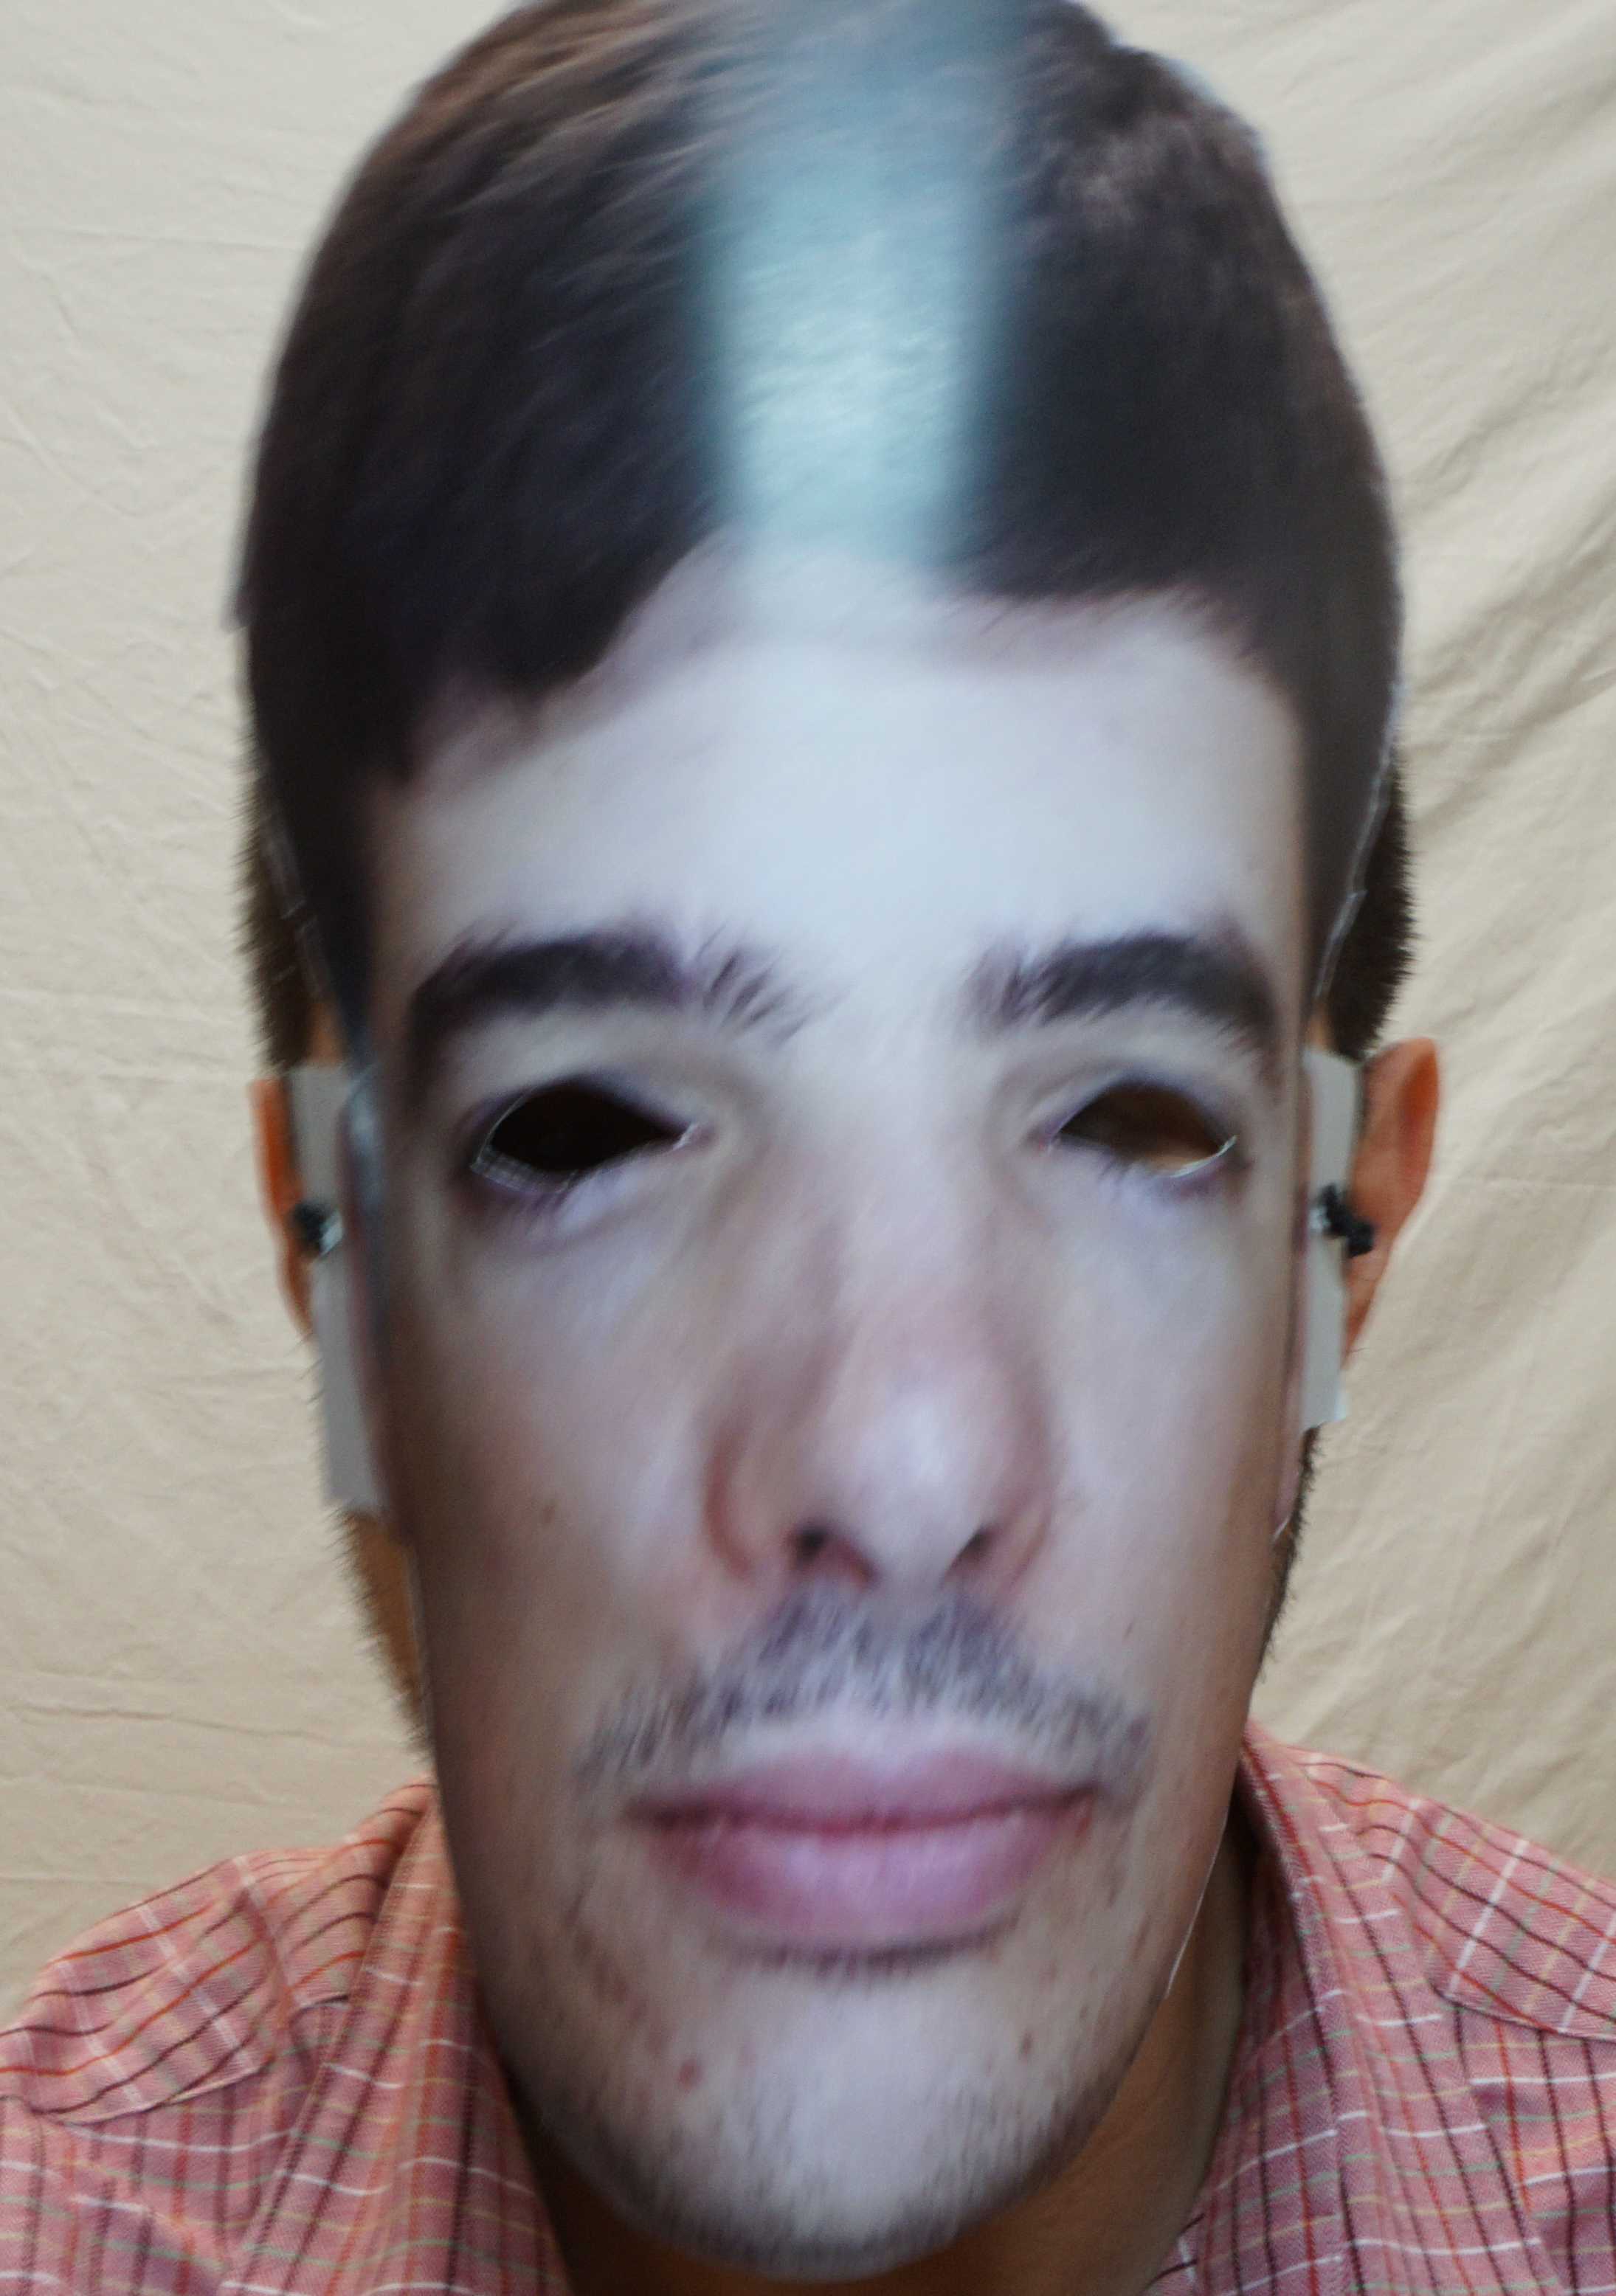
\includegraphics[width=0.18\textwidth]{images_databases/fravrgb/at3-0.JPG} \label{frav_im1-3}}
\subfigure[tablet attack]{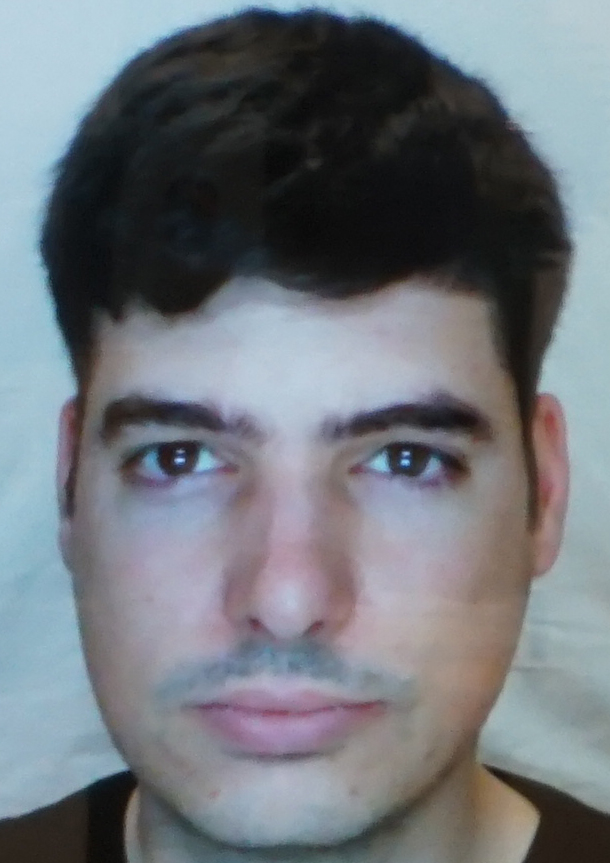
\includegraphics[width=0.18\textwidth]{images_databases/fravrgb/at4-0.JPG} \label{frav_im1-4}}
\subfigure[real user]{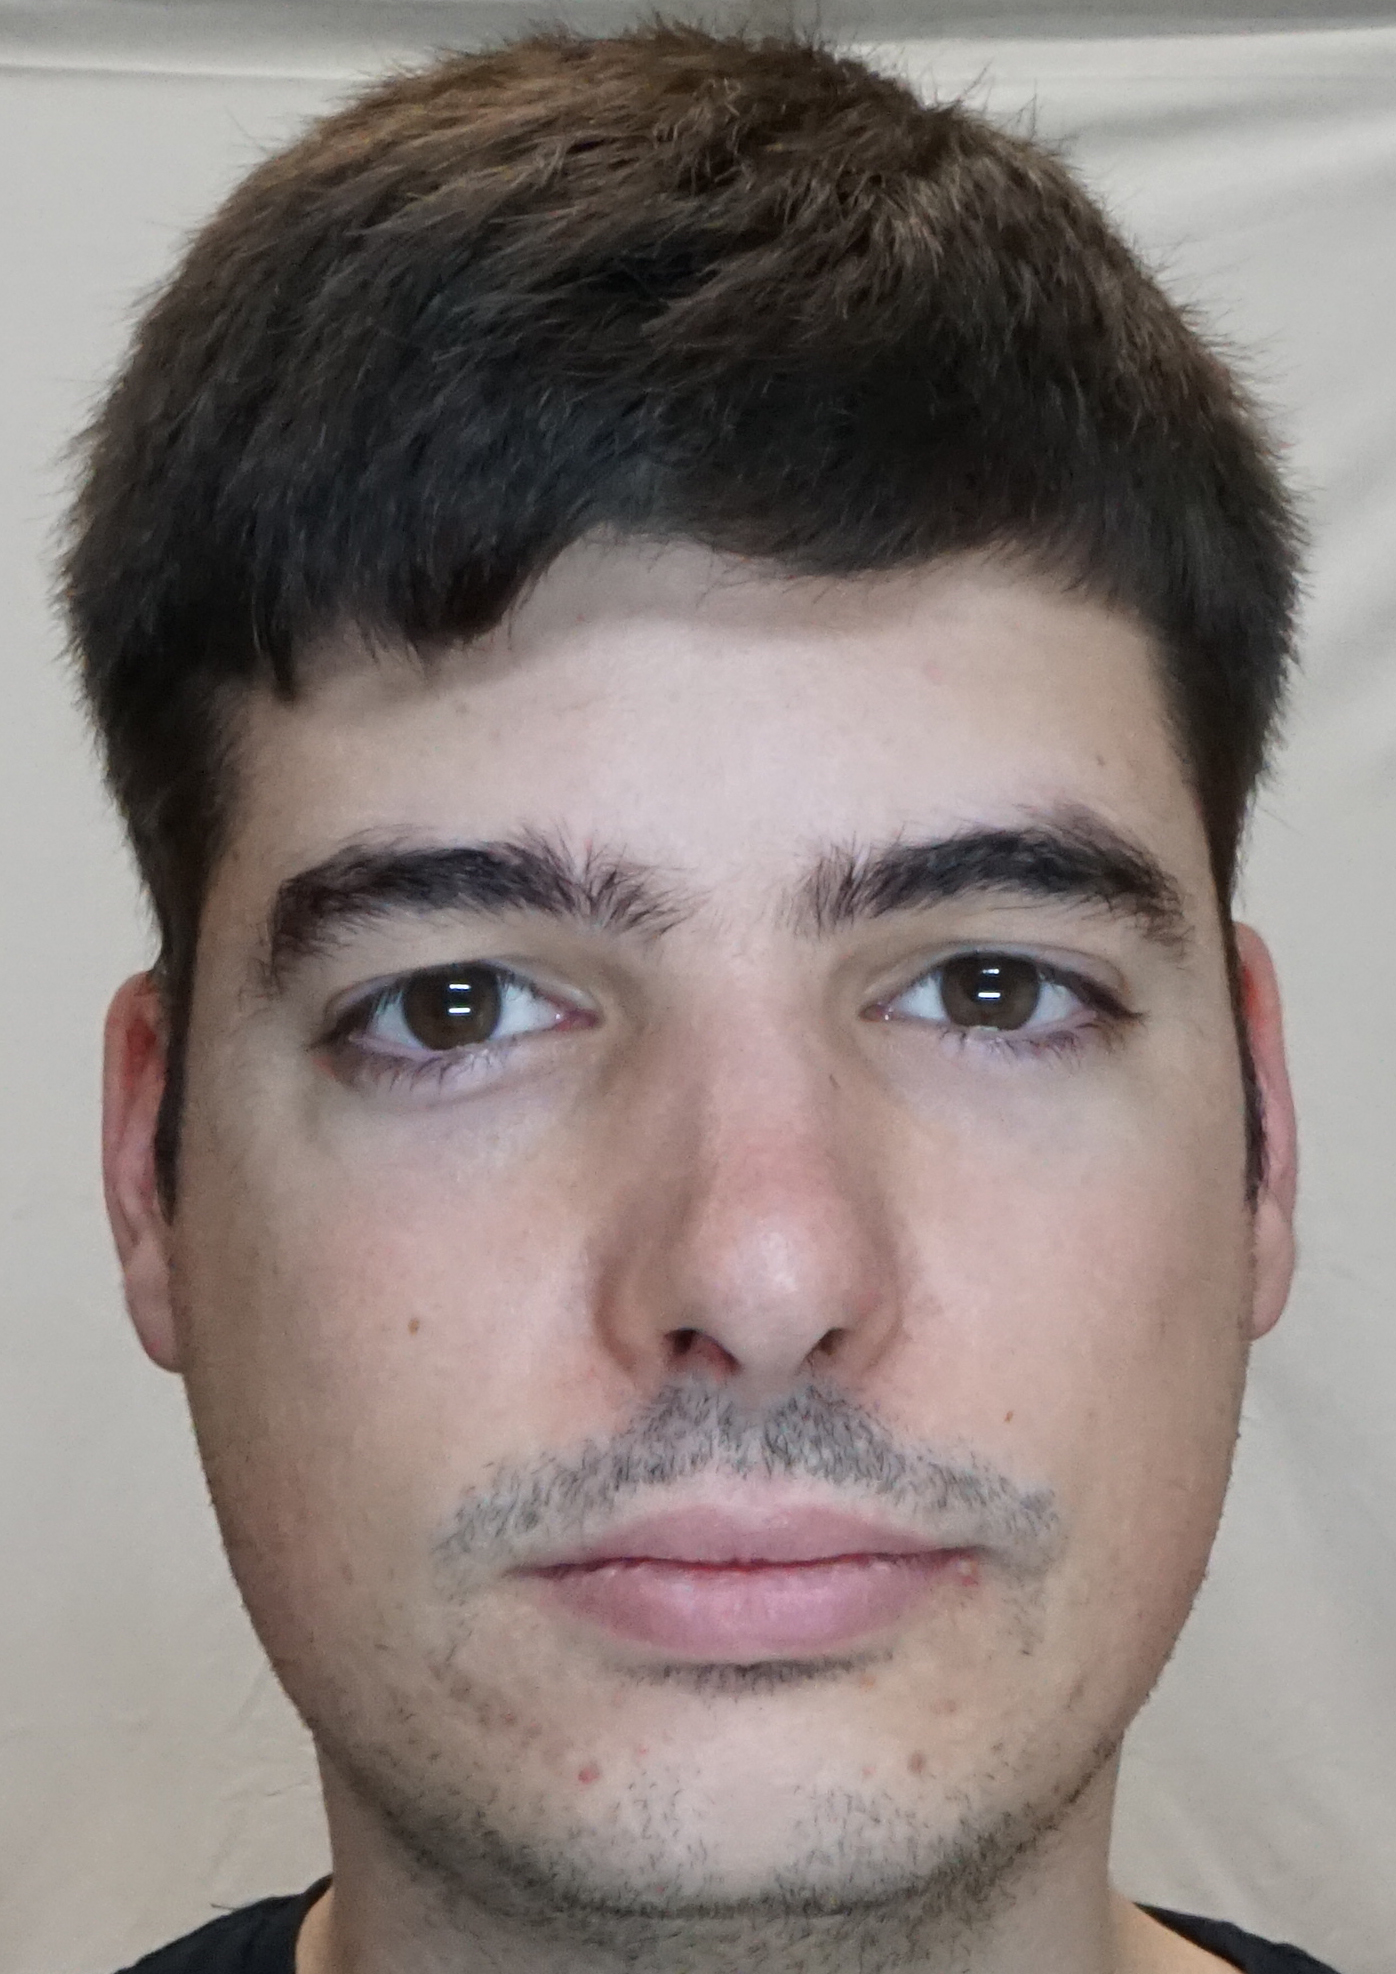
\includegraphics[width=0.18\textwidth]{images_databases/fravrgb/real0.JPG} \label{frav_im1-5}}

\caption{Four attacks and real user from RGB FRAV database } \label{fig:RGB-frav1}
\end{figure}

\begin{figure}[htb]
\centering
\subfigure[printed image attack]{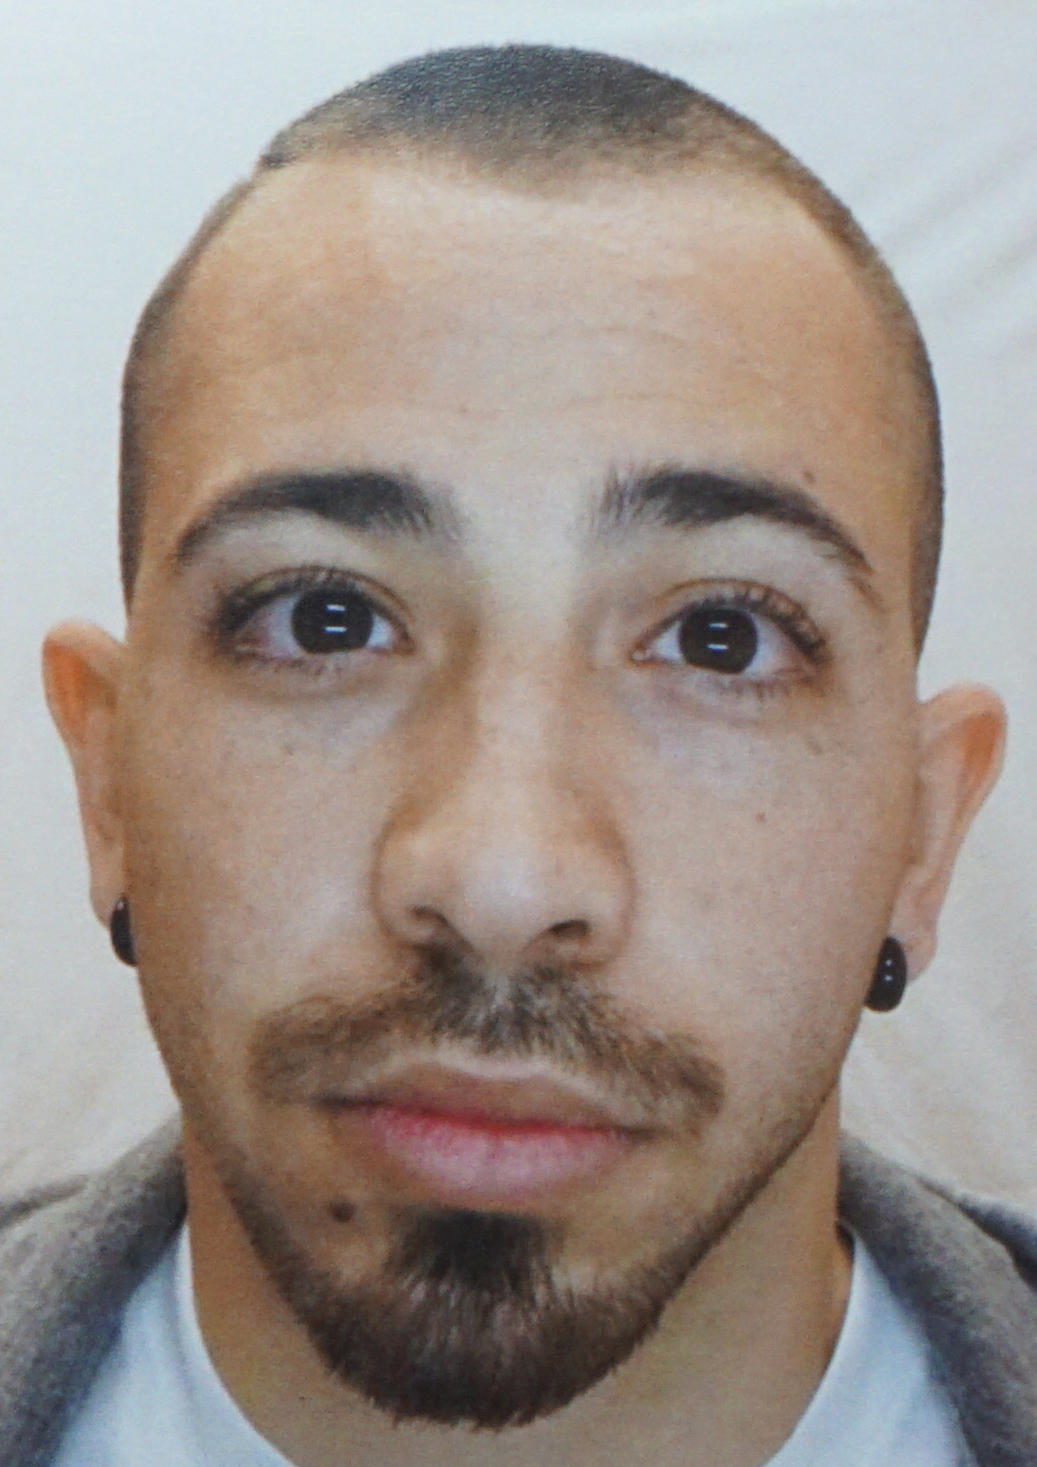
\includegraphics[width=0.18\textwidth]{images_databases/fravrgb/at1-1.JPG} \label{frav_im2-1} }
\subfigure[mask attack]{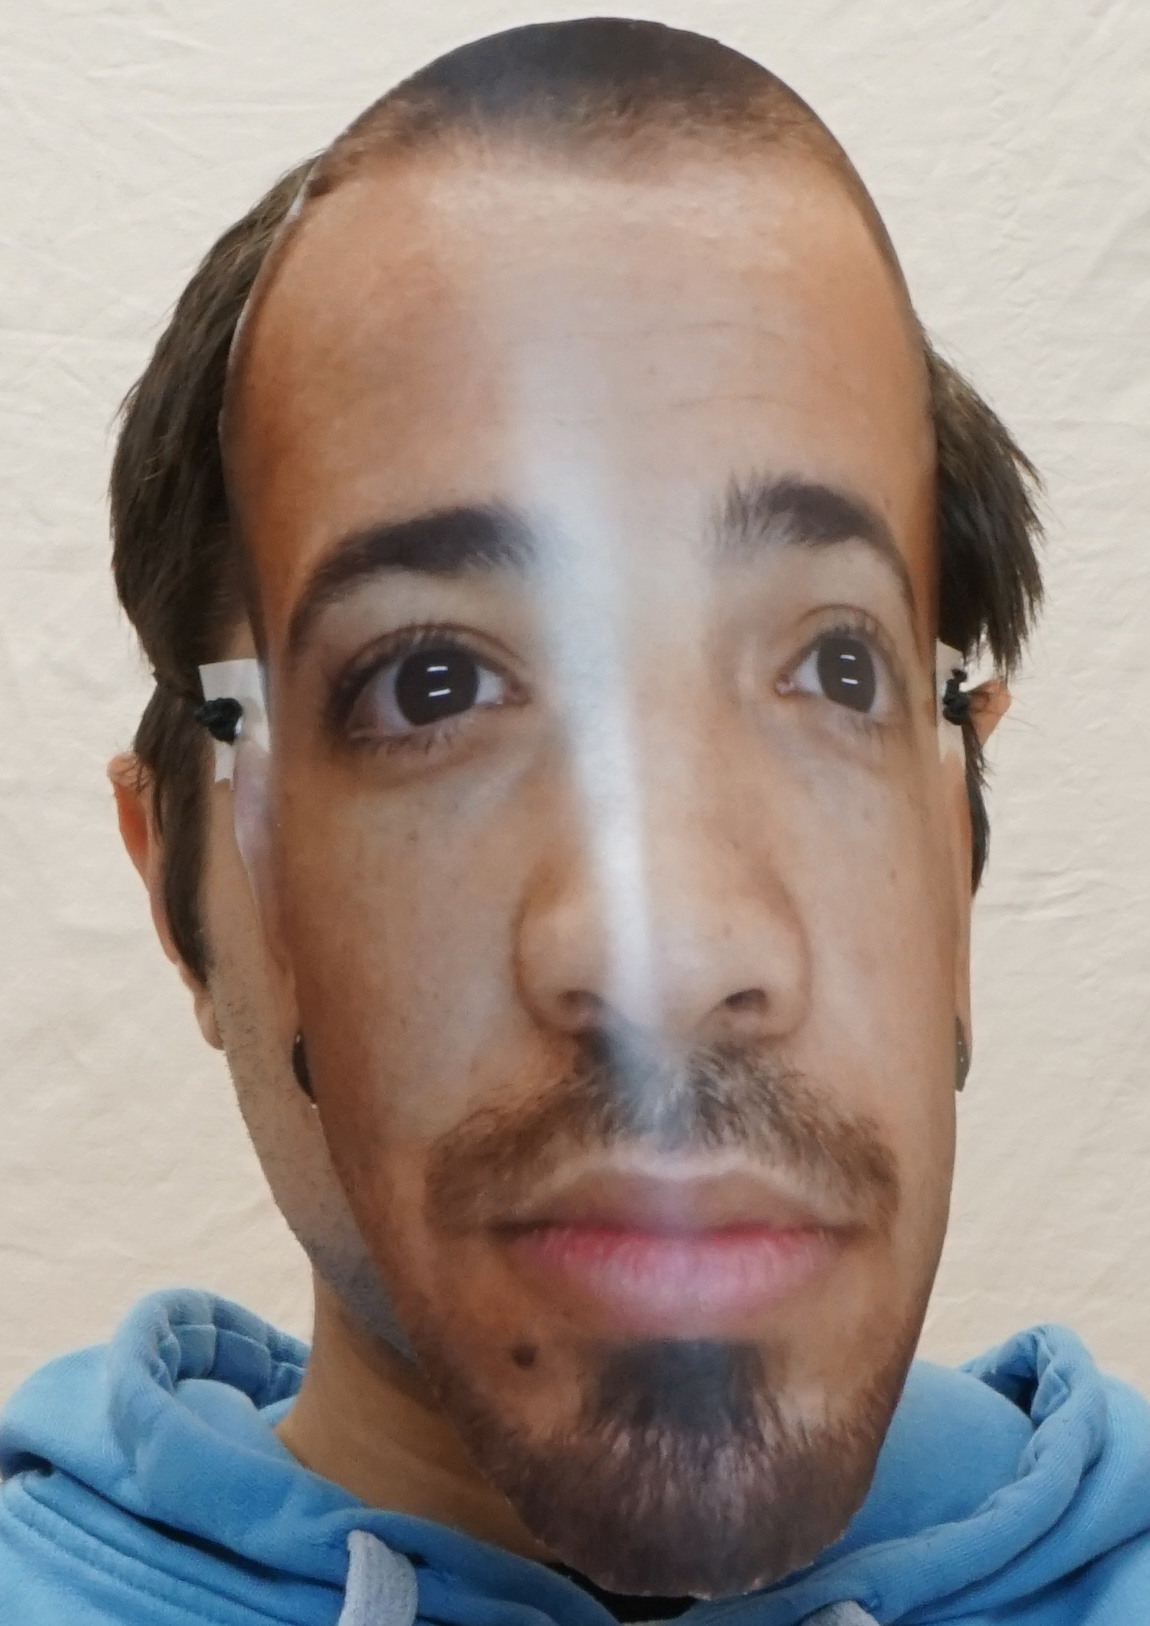
\includegraphics[width=0.18\textwidth]{images_databases/fravrgb/at2-1.JPG} \label{frav_im2-2}}
\subfigure[eye mask attack]{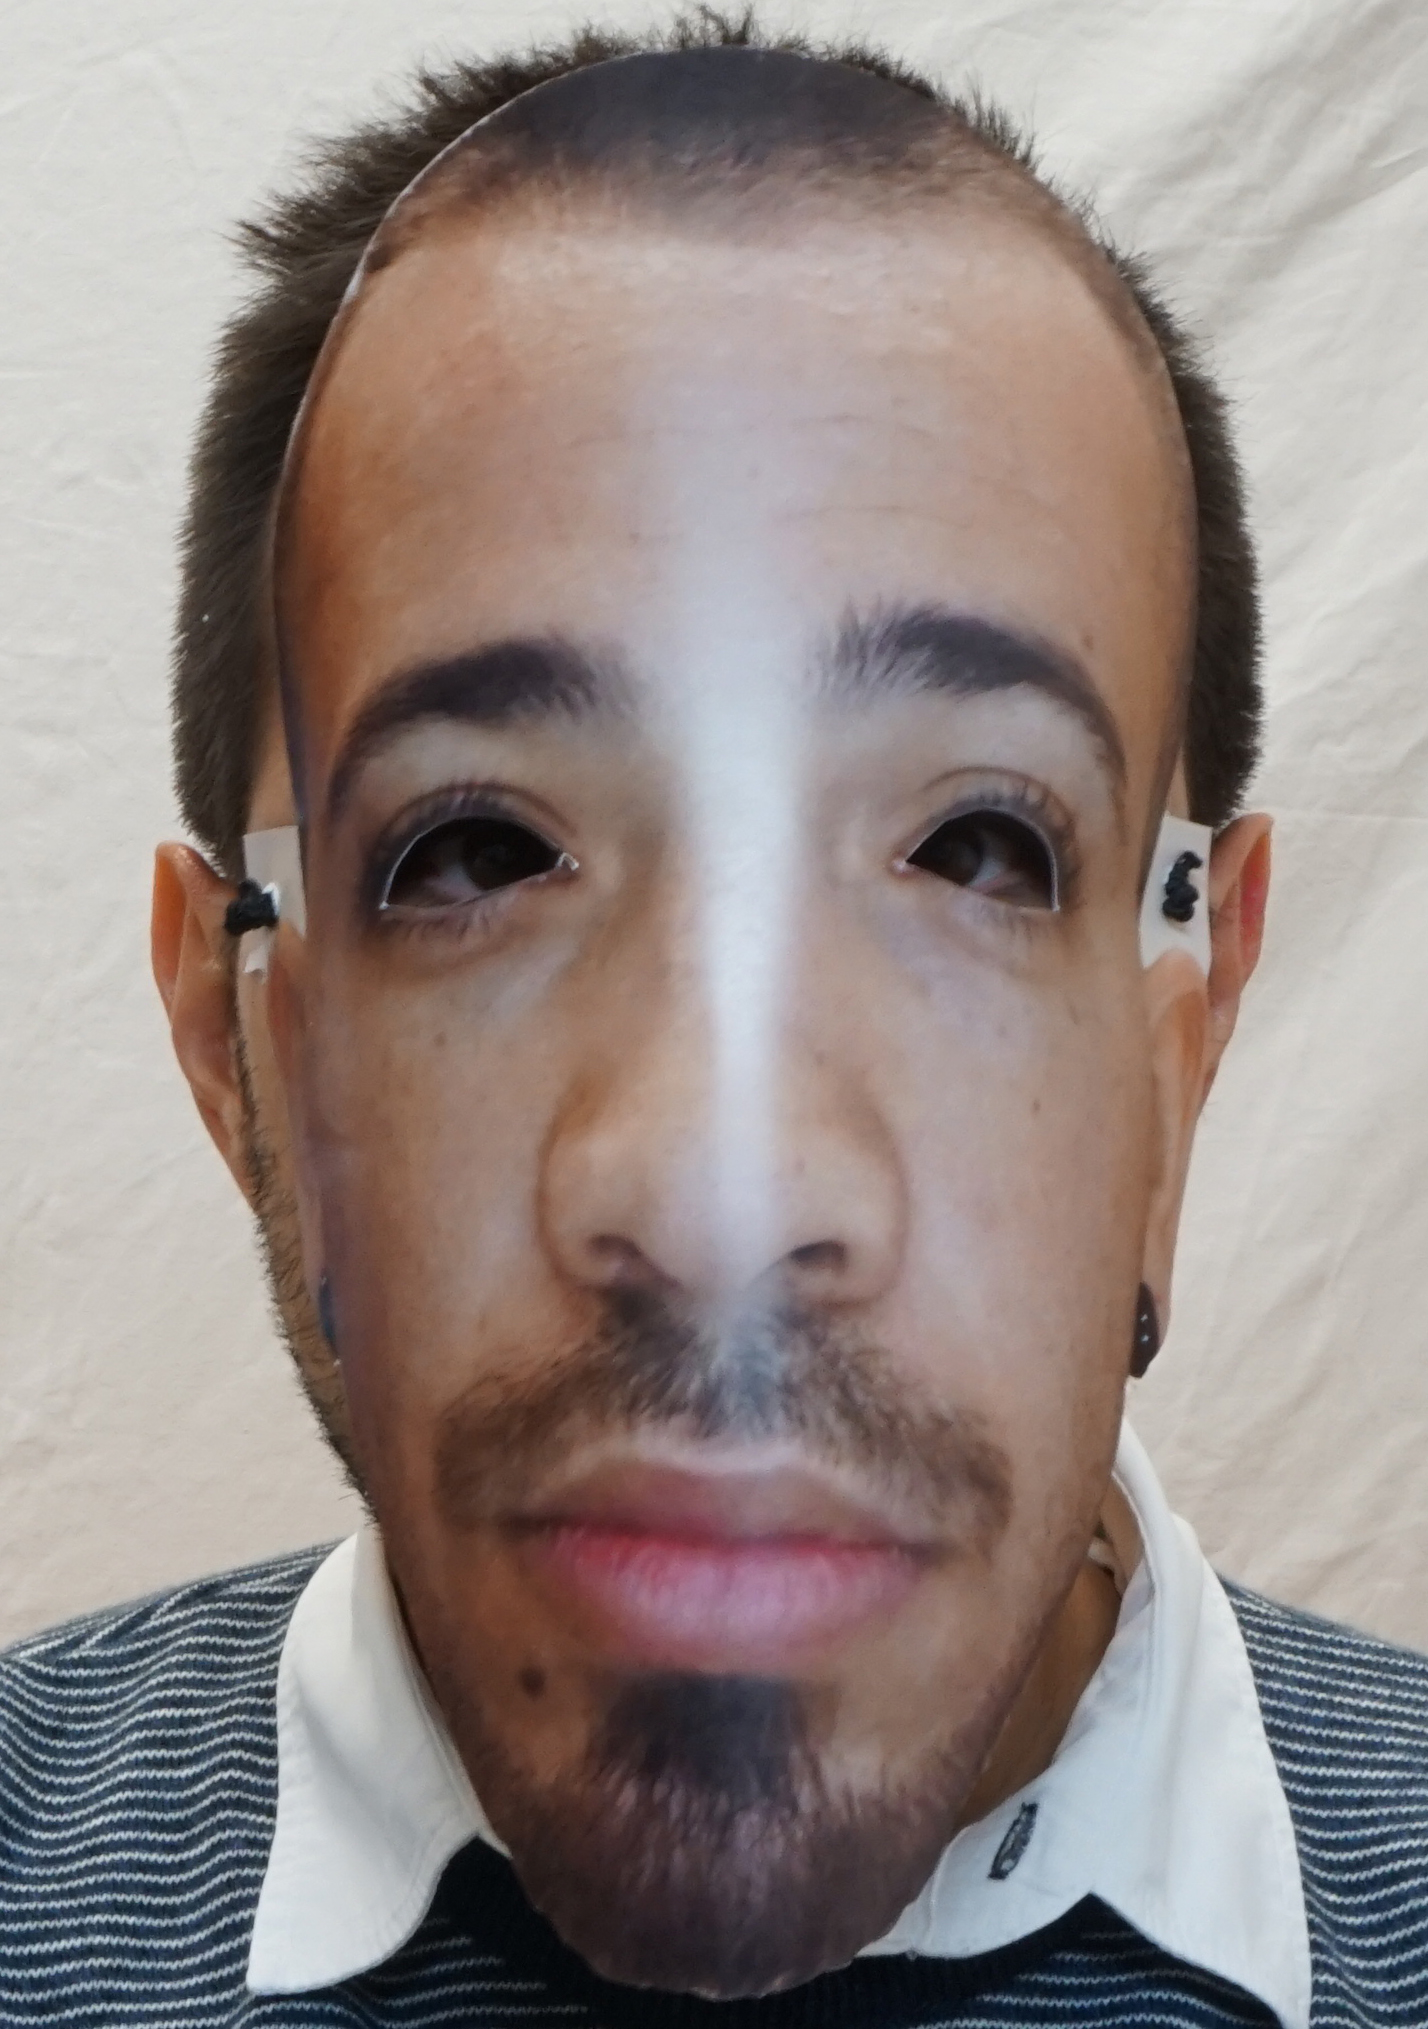
\includegraphics[width=0.18\textwidth]{images_databases/fravrgb/at3-1.JPG} \label{frav_im2-3}}
\subfigure[tablet attack]{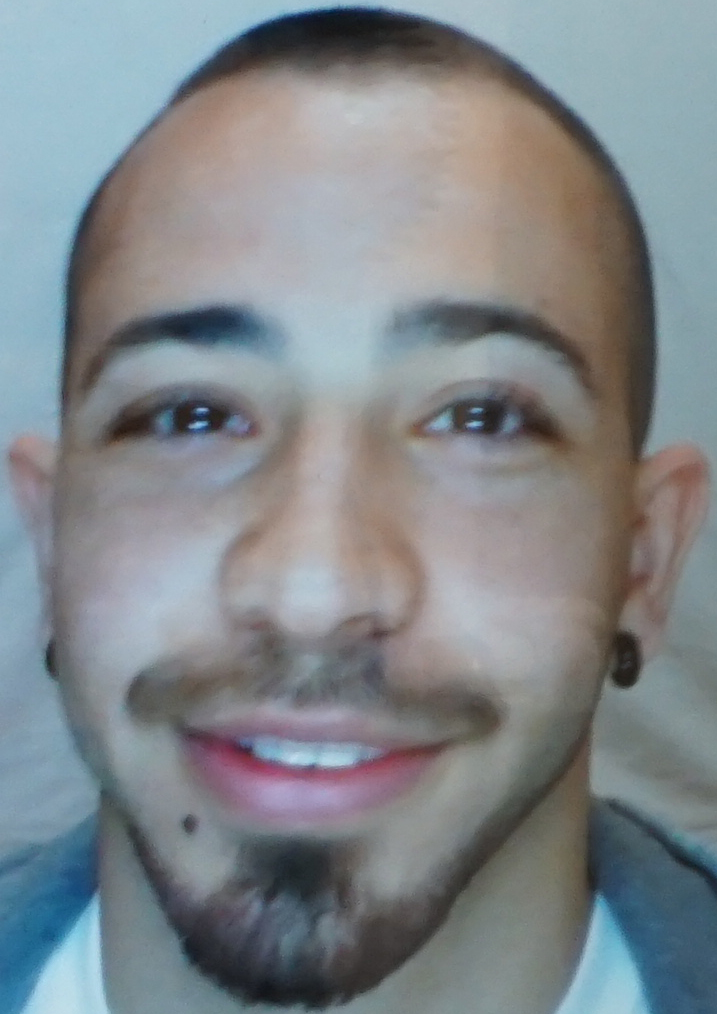
\includegraphics[width=0.18\textwidth]{images_databases/fravrgb/at4-1.JPG} \label{frav_im2-4}}
\subfigure[real user]{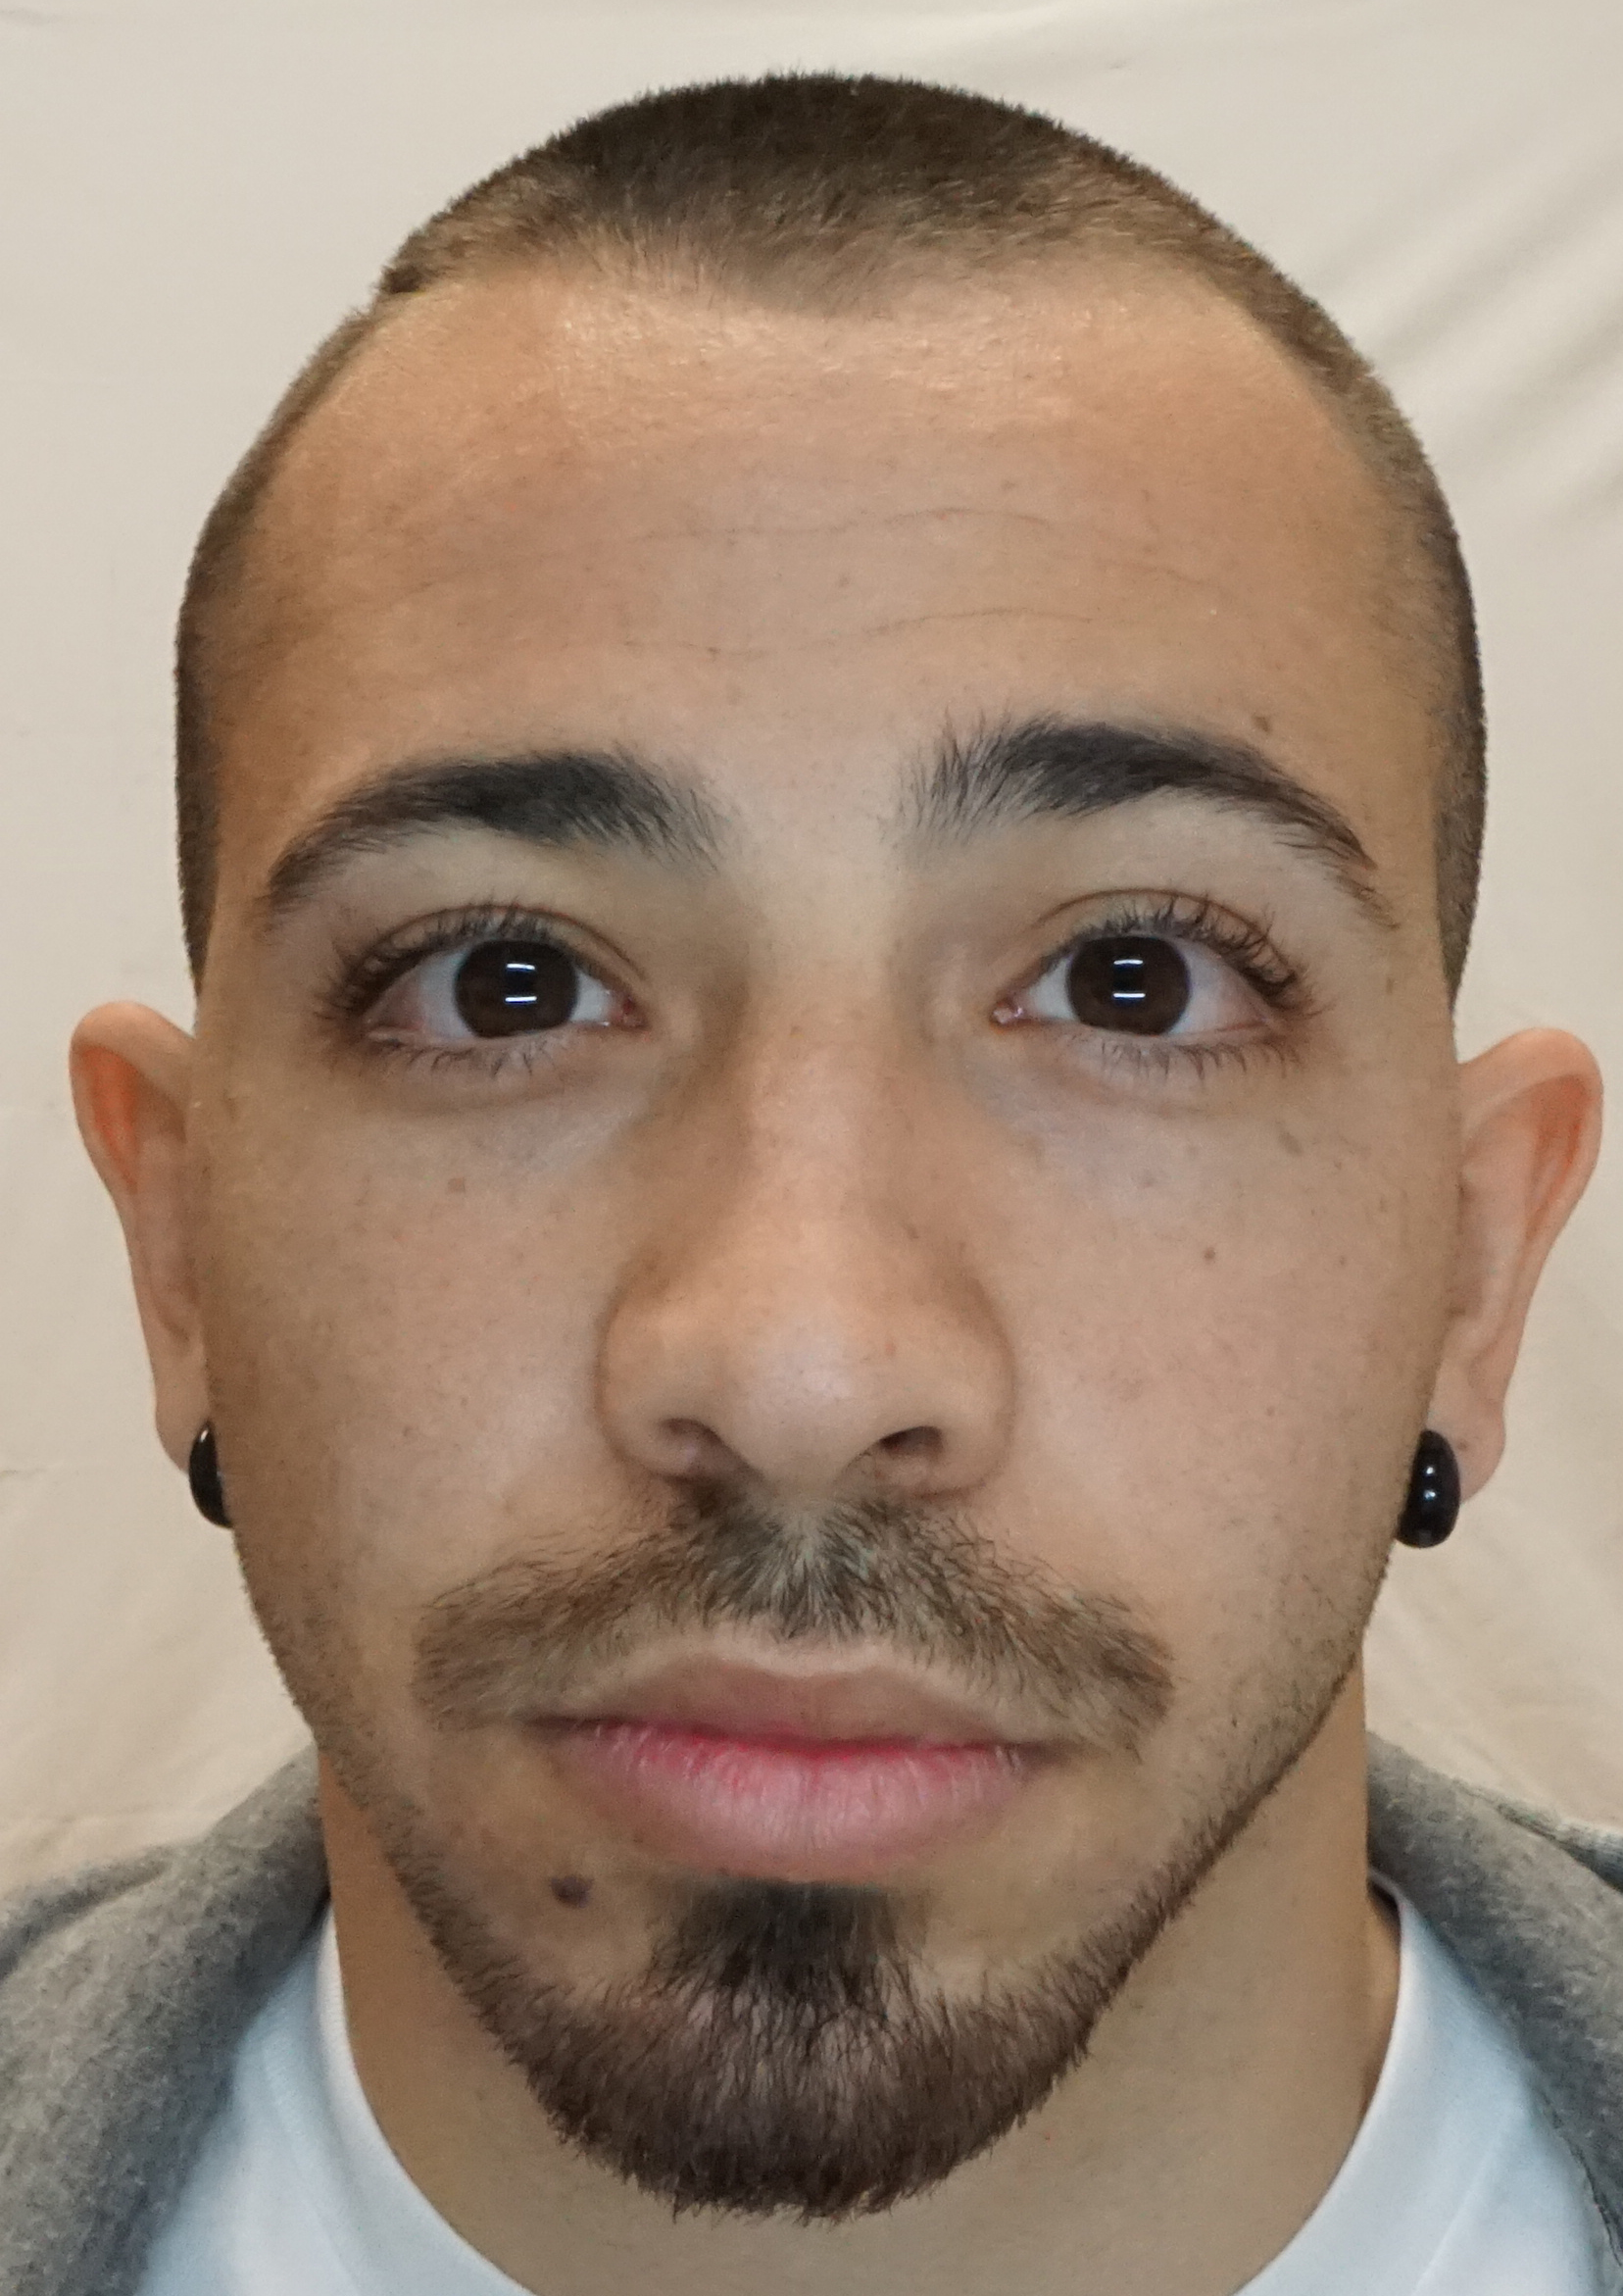
\includegraphics[width=0.18\textwidth]{images_databases/fravrgb/real1.JPG} \label{frav_im2-5}}

\caption{Four attacks and real user from RGB FRAV database } \label{fig:RGB-frav2}
\end{figure}

As could be seen in figure \ref{fig:RGB-frav1} and figure \ref{fig:RGB-frav2}, five different classes composes this database. One class is the real user class and the other four classes are four spoofing attacks per user:\\

\begin{itemize}
 \item Original images of people represented in figure \ref{frav_im1-4}.
 \item Images of people printed (attack) represented in figure \ref{frav_im1-1} and figure \ref{frav_im2-1}.
 \item Images of people with a mask (attack)represented in figure \ref{frav_im1-2}and figure \ref{frav_im2-2}.
 \item Images of people with a mask with the eyes cropped (attack)represented in figure \ref{frav_im1-3} and figure \ref{frav_im2-3}
 \item Images of people in a tablet (attack)represented in figure \ref{frav_im1-4} and figure \ref{frav_im2-4}.\\
 \end{itemize}

Images of classes can be found in RGB and NIR (not all RGB images has its corresponding NIR image). Characteristics of FRAV images database are the following ones:\\

\begin{itemize}
 \item There are 939 people in each RGB class or 195 in each NIR class.
\item There is one image per person.
\item Each image has it is own shape.
\item As it real user has all the four attaks, all the classes has the same number of samples.
\item The faces are centred in the image.\\
\end{itemize}

This database is used in two different ways:

\begin{enumerate}
  \item Using only RGB images, where there are 933 people, in which each person would have a genuine image and four attack, so 4665 samples are available.
  \item Using the RGB and NIR images, where there are 195 people which correspond with NIR images and its corresponding images in RGB. 975 samples are available.
\end{enumerate}

If RGB and NIR images are used at the same time, two different methods, for using both types of images together, are used:
\begin{itemize}
\item Characteristic level: adding the NIR image as another layer to RGB image, so the resultant image have hightxweightx4 dimensions (NIR images has one layer because it is a gray scale image and RGB images has tree layers, one per each primary color). The network is feed with the resultant images like other times.
\item Classification level: after the network training and before feeding the classifier, RGB and NIR would be trained separately and its features would be appended as the input of the classifier. 
\end{itemize}

To conclude, this database is going to be used in the three different ways: just RGB images, RGB and NIR images added in characteristic level or classification level.\\ 

When the classes are build, two ways are possible to be done: the first one where real people are one class (positive) and the different attacks are other class (negatives), so two classes have been used; and the second way where each attacks correspond with a class, so five classes (4 attacks and 1 real) have been used.\\


\subsection{CASIA dataset}
The CASIA Face Anti-Spoofing database is a database from the Chinese Academy of Sciences Centre for Biometrics and Security Research (CASIA-CBSR) \cite{Casiadatbase}.


In the same way as FRAV dataset, this database is formed by real or genuine images of people and three different attacks of the same people:

\begin{itemize}
 \item Images of people printed (attack).
 \item Images of people with a mask (attack).
 \item Images of people with a mask with the eyes cropped (attack).
 \end{itemize}


\begin{itemize}
\item There are 939 people in each RGB class or 195 in NIR class.
\item There is one image per person.
\item The size of each image is 720x1280 pixels.
\item The faces in images are in the center of the image.\\
\item Images are RGB.
\end{itemize}


Two people of Casia database could be seen in figure \ref{fig:casia1} and figure \ref{fig:casia2}, where three attacks types could be seen with the real user of both examples.

\begin{figure}[htb]
\centering
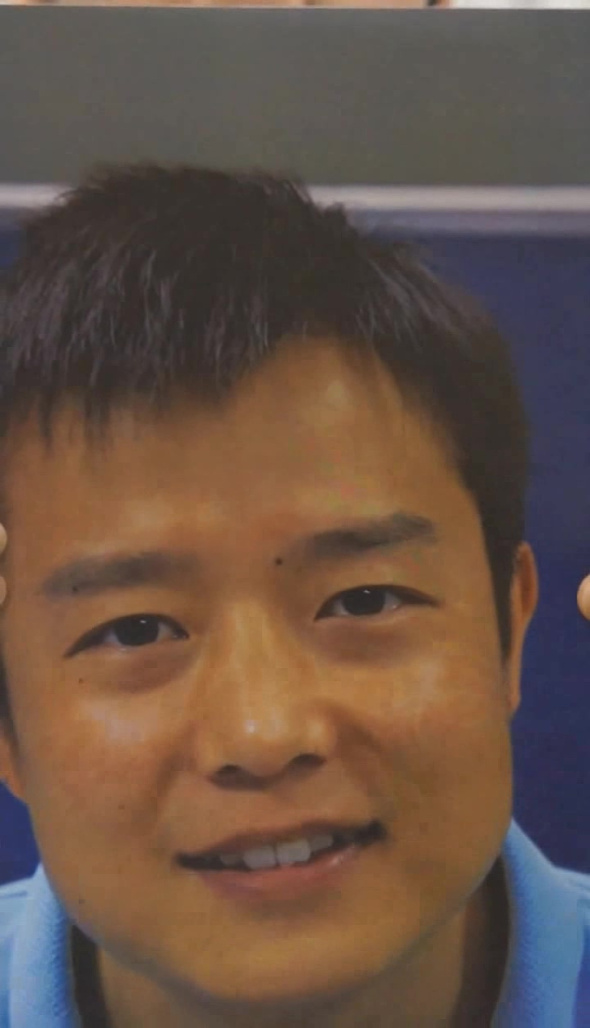
\includegraphics[width=0.2\textwidth]{images_databases/casia/at1-2.jpg}
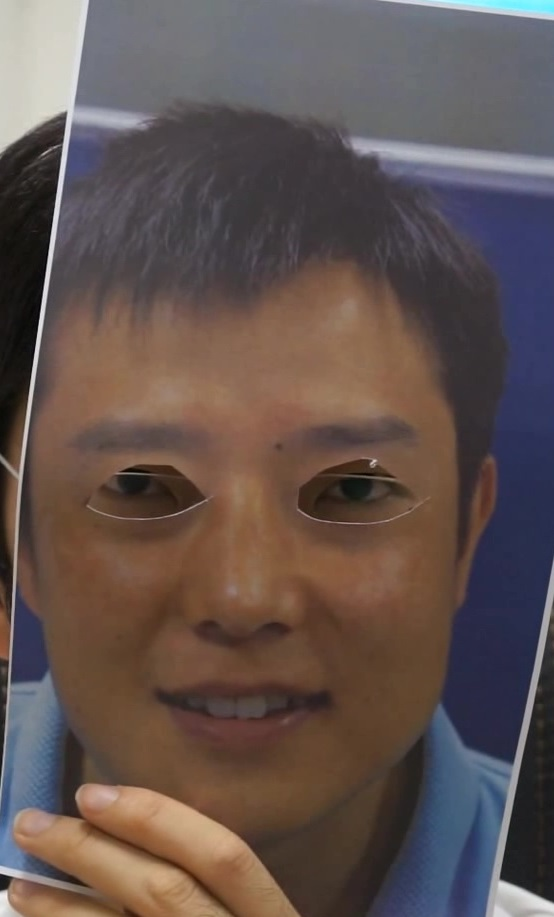
\includegraphics[width=0.2\textwidth]{images_databases/casia/at2-2.jpg}
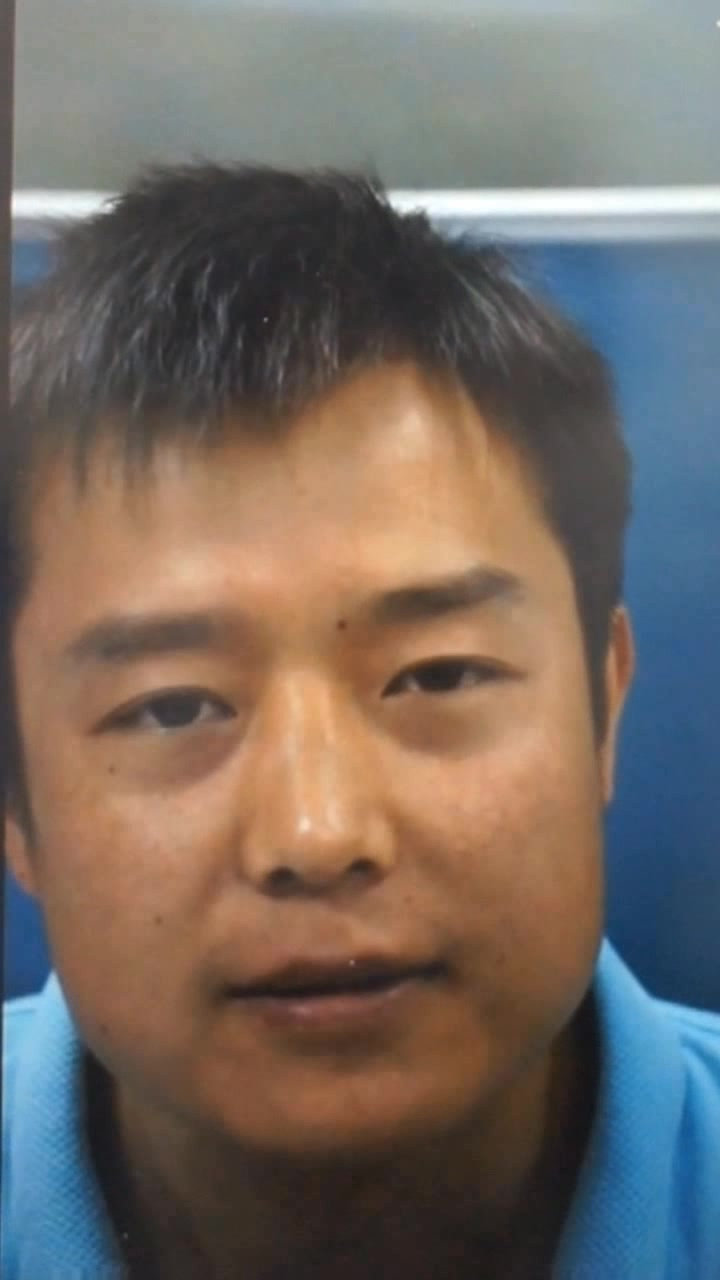
\includegraphics[width=0.2\textwidth]{images_databases/casia/at3-2.jpg}
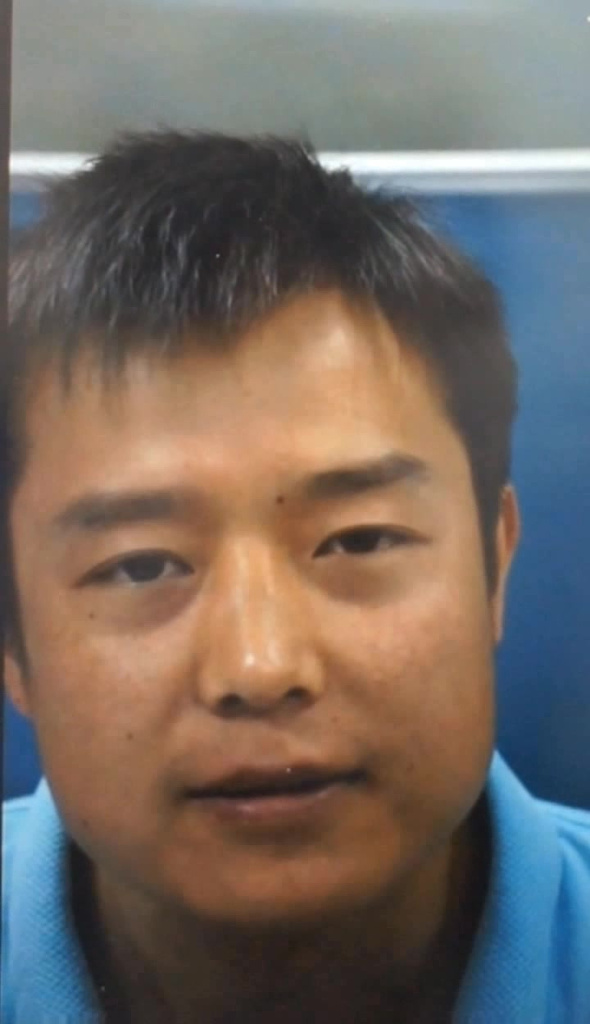
\includegraphics[width=0.2\textwidth]{images_databases/casia/real2.jpg}

\caption{Three attacks and real user from casia database } \label{fig:casia2}
\end{figure}

\begin{figure}[htb]
\centering
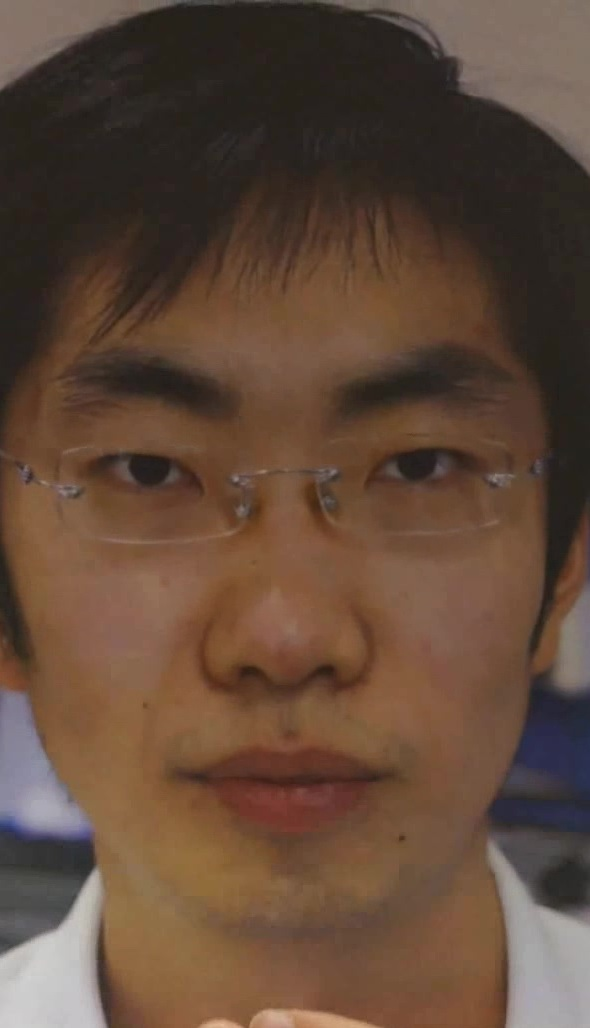
\includegraphics[width=0.2\textwidth]{images_databases/casia/at1-1.jpg}
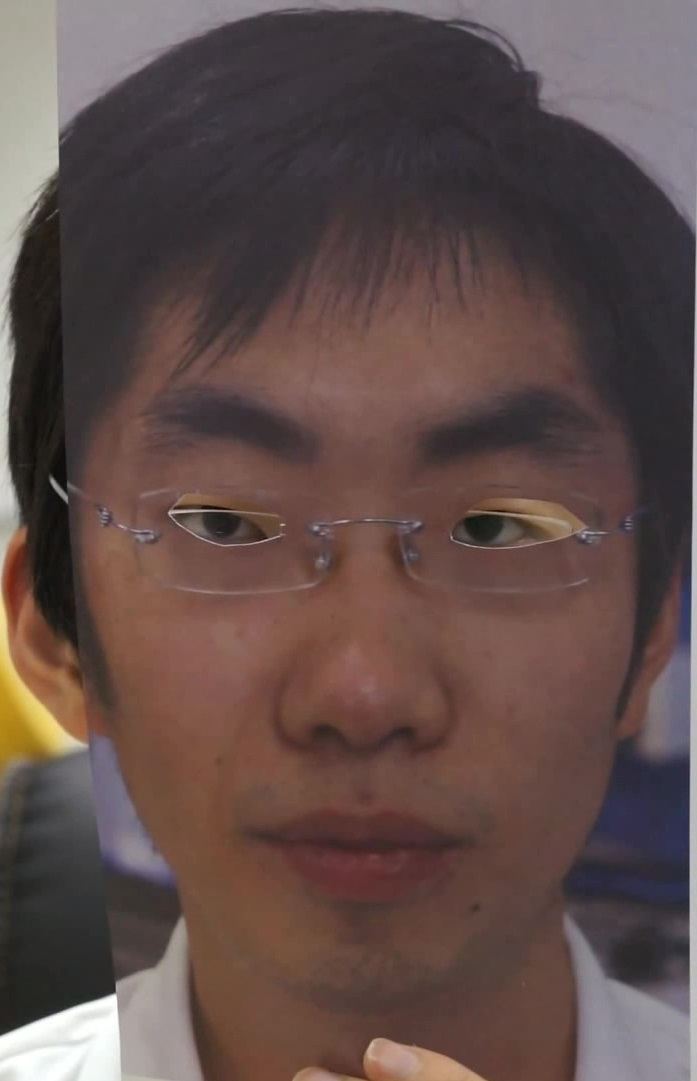
\includegraphics[width=0.2\textwidth]{images_databases/casia/at2-1.jpg}
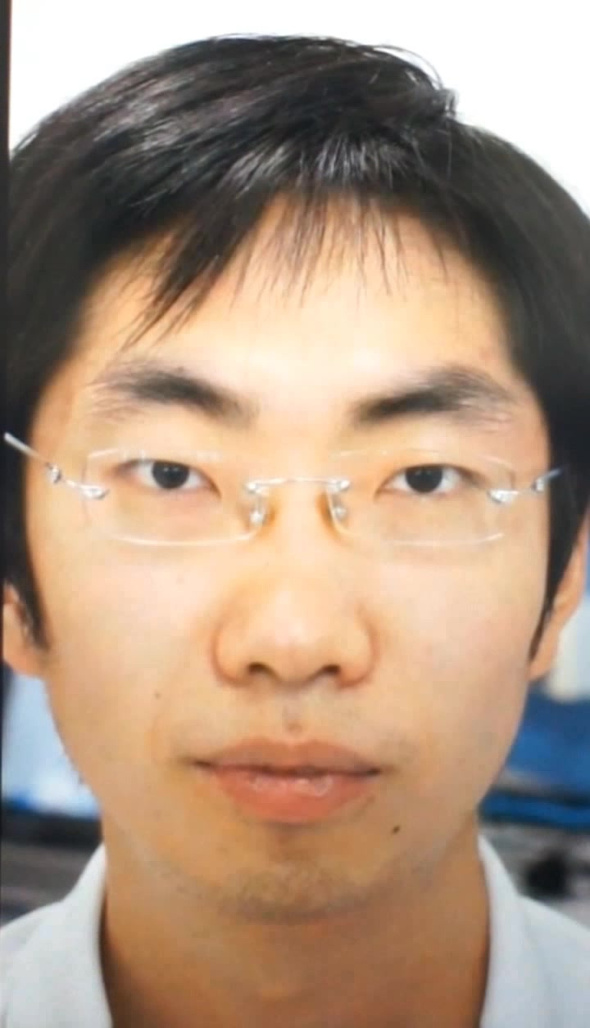
\includegraphics[width=0.2\textwidth]{images_databases/casia/at3-1.jpg}
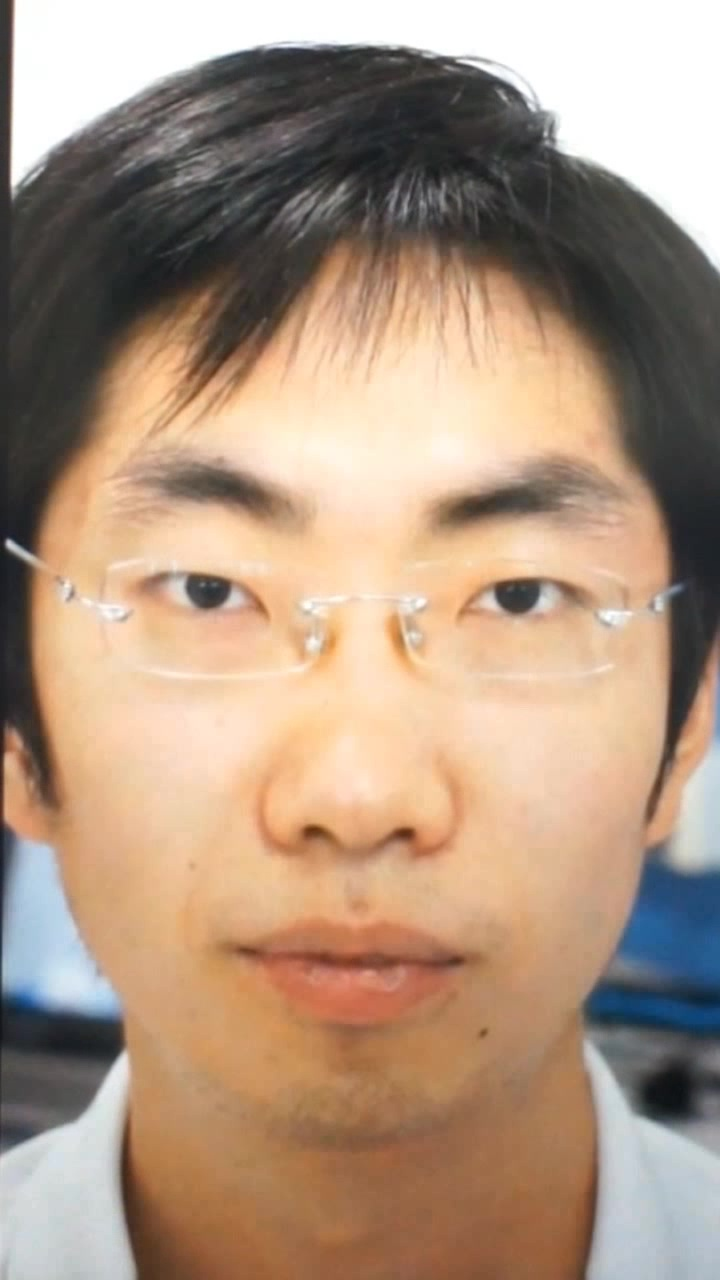
\includegraphics[width=0.2\textwidth]{images_databases/casia/real1.jpg}

\caption{Three attacks and real user from casia database } \label{fig:casia1}
\end{figure}

\subsection{MSU - MFSD database}
The MSU Mobile Face Spoofing Database (MFSD) is a video face anti-spoofing database although for this work just images have been used.\\

The database consist on users and attacks of the same people:\\
\begin{itemize}
\item Genuine users
\item
\end{itemize}

The characteristics of the database are the following ones:\\

\begin{itemize}
\item 35 images per attack or genuine user.
\item Images are RGB.
\item Faces are centered in images.
\item The size of each image are not equal. Approximately images are 300px heigh and 335px width.
\end{itemize}

In figure \ref{fig:mfsd} and figure \ref{fig:mfsd2} It is posible to see the three attacks and the real user.\\

\begin{figure}[htb]
\centering
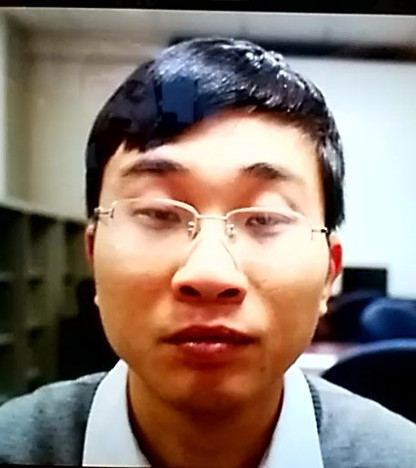
\includegraphics[width=0.2\textwidth]{images_databases/MFSD/at1-1.jpg}
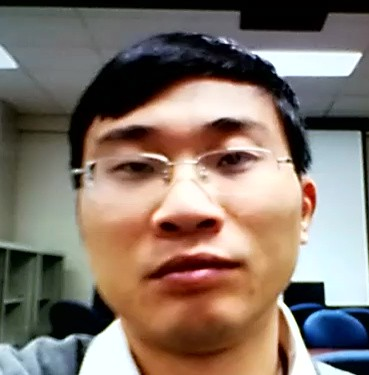
\includegraphics[width=0.2\textwidth]{images_databases/MFSD/at2-1.jpg}
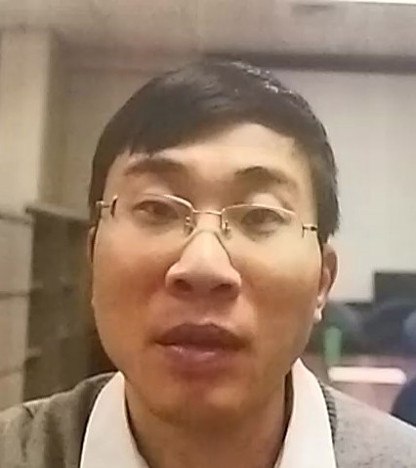
\includegraphics[width=0.2\textwidth]{images_databases/MFSD/at3-1.jpg}
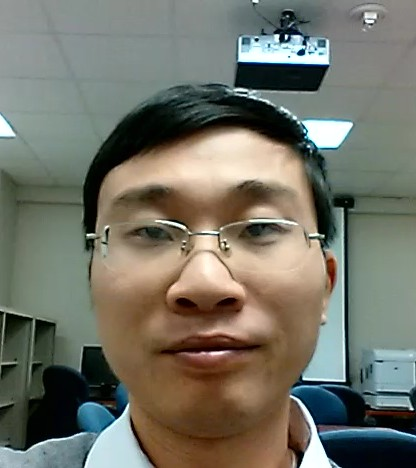
\includegraphics[width=0.2\textwidth]{images_databases/MFSD/1.jpg}
\caption{Three attacks and real user from a user of MFSD database } \label{fig:mfsd}
\end{figure}

\begin{figure}[htb]
\centering
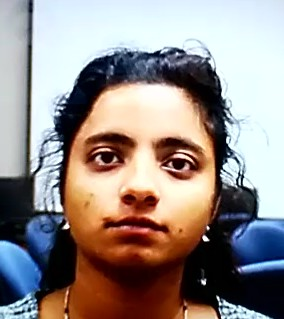
\includegraphics[width=0.2\textwidth]{images_databases/MFSD/at1-2.jpg}
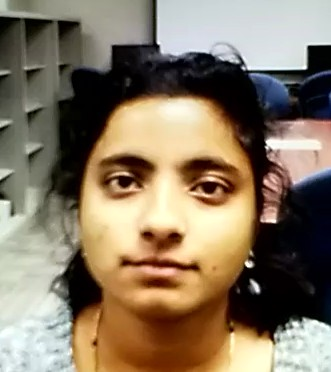
\includegraphics[width=0.2\textwidth]{images_databases/MFSD/at2-2.jpg}
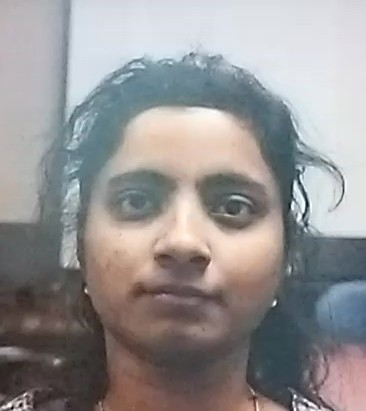
\includegraphics[width=0.2\textwidth]{images_databases/MFSD/at3-2.jpg}
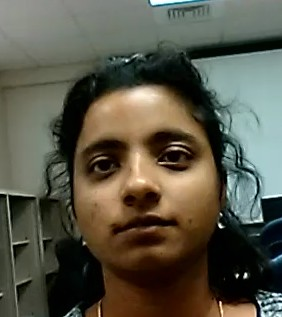
\includegraphics[width=0.2\textwidth]{images_databases/MFSD/2.jpg}
\caption{Three attacks and real user from a user of MFSD database } \label{fig:mfsd2}
\end{figure}
